\chapter{Numerical Time Integration of Partial/Ordinary Differential Equations}

\section{Introduction}

Many engineering problems are described as either a partial differential equation (PDE) or ordinary differential equation (ODE). A broad class of important problems is called the ``Initial Value Problem'' (IVP). Take for example the continuity equation in semiconductors, which is given as\begin{IEEEeqnarray}{rCl}
\frac{\partial n}{\partial t} & = & -\text{div}\left(\bm{J}\right) + G_\text{n} - R_\text{n} \label{eq:continuityEqn}
\end{IEEEeqnarray}where $n$ is the carrier concentration, $\bm{J}$ is the current density flowing through the semiconductor, $G_\text{n}$ and $R_\text{n}$ are the rates of carrier generation and recombination due to generation and recombination processes, respectively. The IVP would be as follows: assume that at time, $t=0$, the carrier concentration is $n(t=0)={0}$ and we want to find the time-dependent profile of the carrier concentration, $n(t)$.

In general, the PDE is more complicated than that in Equation~(\ref{eq:continuityEqn}), and the time derivative or slope function is denoted as $\dot{y}(t)=f(t, y)$, where $y(t)$ is the quantity we are trying to solve for, having the initial condition $y(t=0)=y_{0}$.

\section{The Forward (Explicit) Euler Method}

One method to obtain $y(t)$ from $f(t,y)$ and $y_{0}$ is to use the forward Euler method. First, the time range over which to determine $y(t)$ is discretized into a uniform grid. The time difference between each grid point, $\Delta t=h$ is called the \emph{time step}. $y(t)$ is then iteratively calculated (starting at $y_{0}$) using the formula\begin{IEEEeqnarray}{rCl}
y(t+h) & = & y(t) + hf(t,y(t)) \label{eq:compExEuler}
\end{IEEEeqnarray}Mathematically, the Equation~(\ref{eq:compExEuler}) is unwieldy and we simplify the expression using $y_{n+1}=y(t+h)$ and $y_{n}=y(t)$, which gives\begin{IEEEeqnarray}{rCl}
y_{n+1} & = & y_{n} + hf(t,y_{n}) \label{eq:simpExEuler}
\end{IEEEeqnarray}

\subsection{Example 1: Solutions with Persistent Oscillations}

Consider the function $y(t) = \sin (t)$ and its time derivative, $\dot{y}(t) = \cos (t)$. The numerical solution for different time steps are plotted in Fig.~\ref{fig:IVP1}. As clearly seen, the error reduces with the size of the time step---a smaller time step returns a numerical result that is closer to the ideal solution.

\subsection{Example 2: Solutions with Damped Relaxations}

Another commonly observed function is $y(t) = \exp(-t)$ and its time derivative, $\dot{y}(t) = -\exp(-t)$. The numerical solution for different time steps are plotted in Fig.~\ref{fig:IVP2}. As clearly seen, the error also reduces with the size of the time step.\afterpage{
\begin{figure}[!t]
\centering
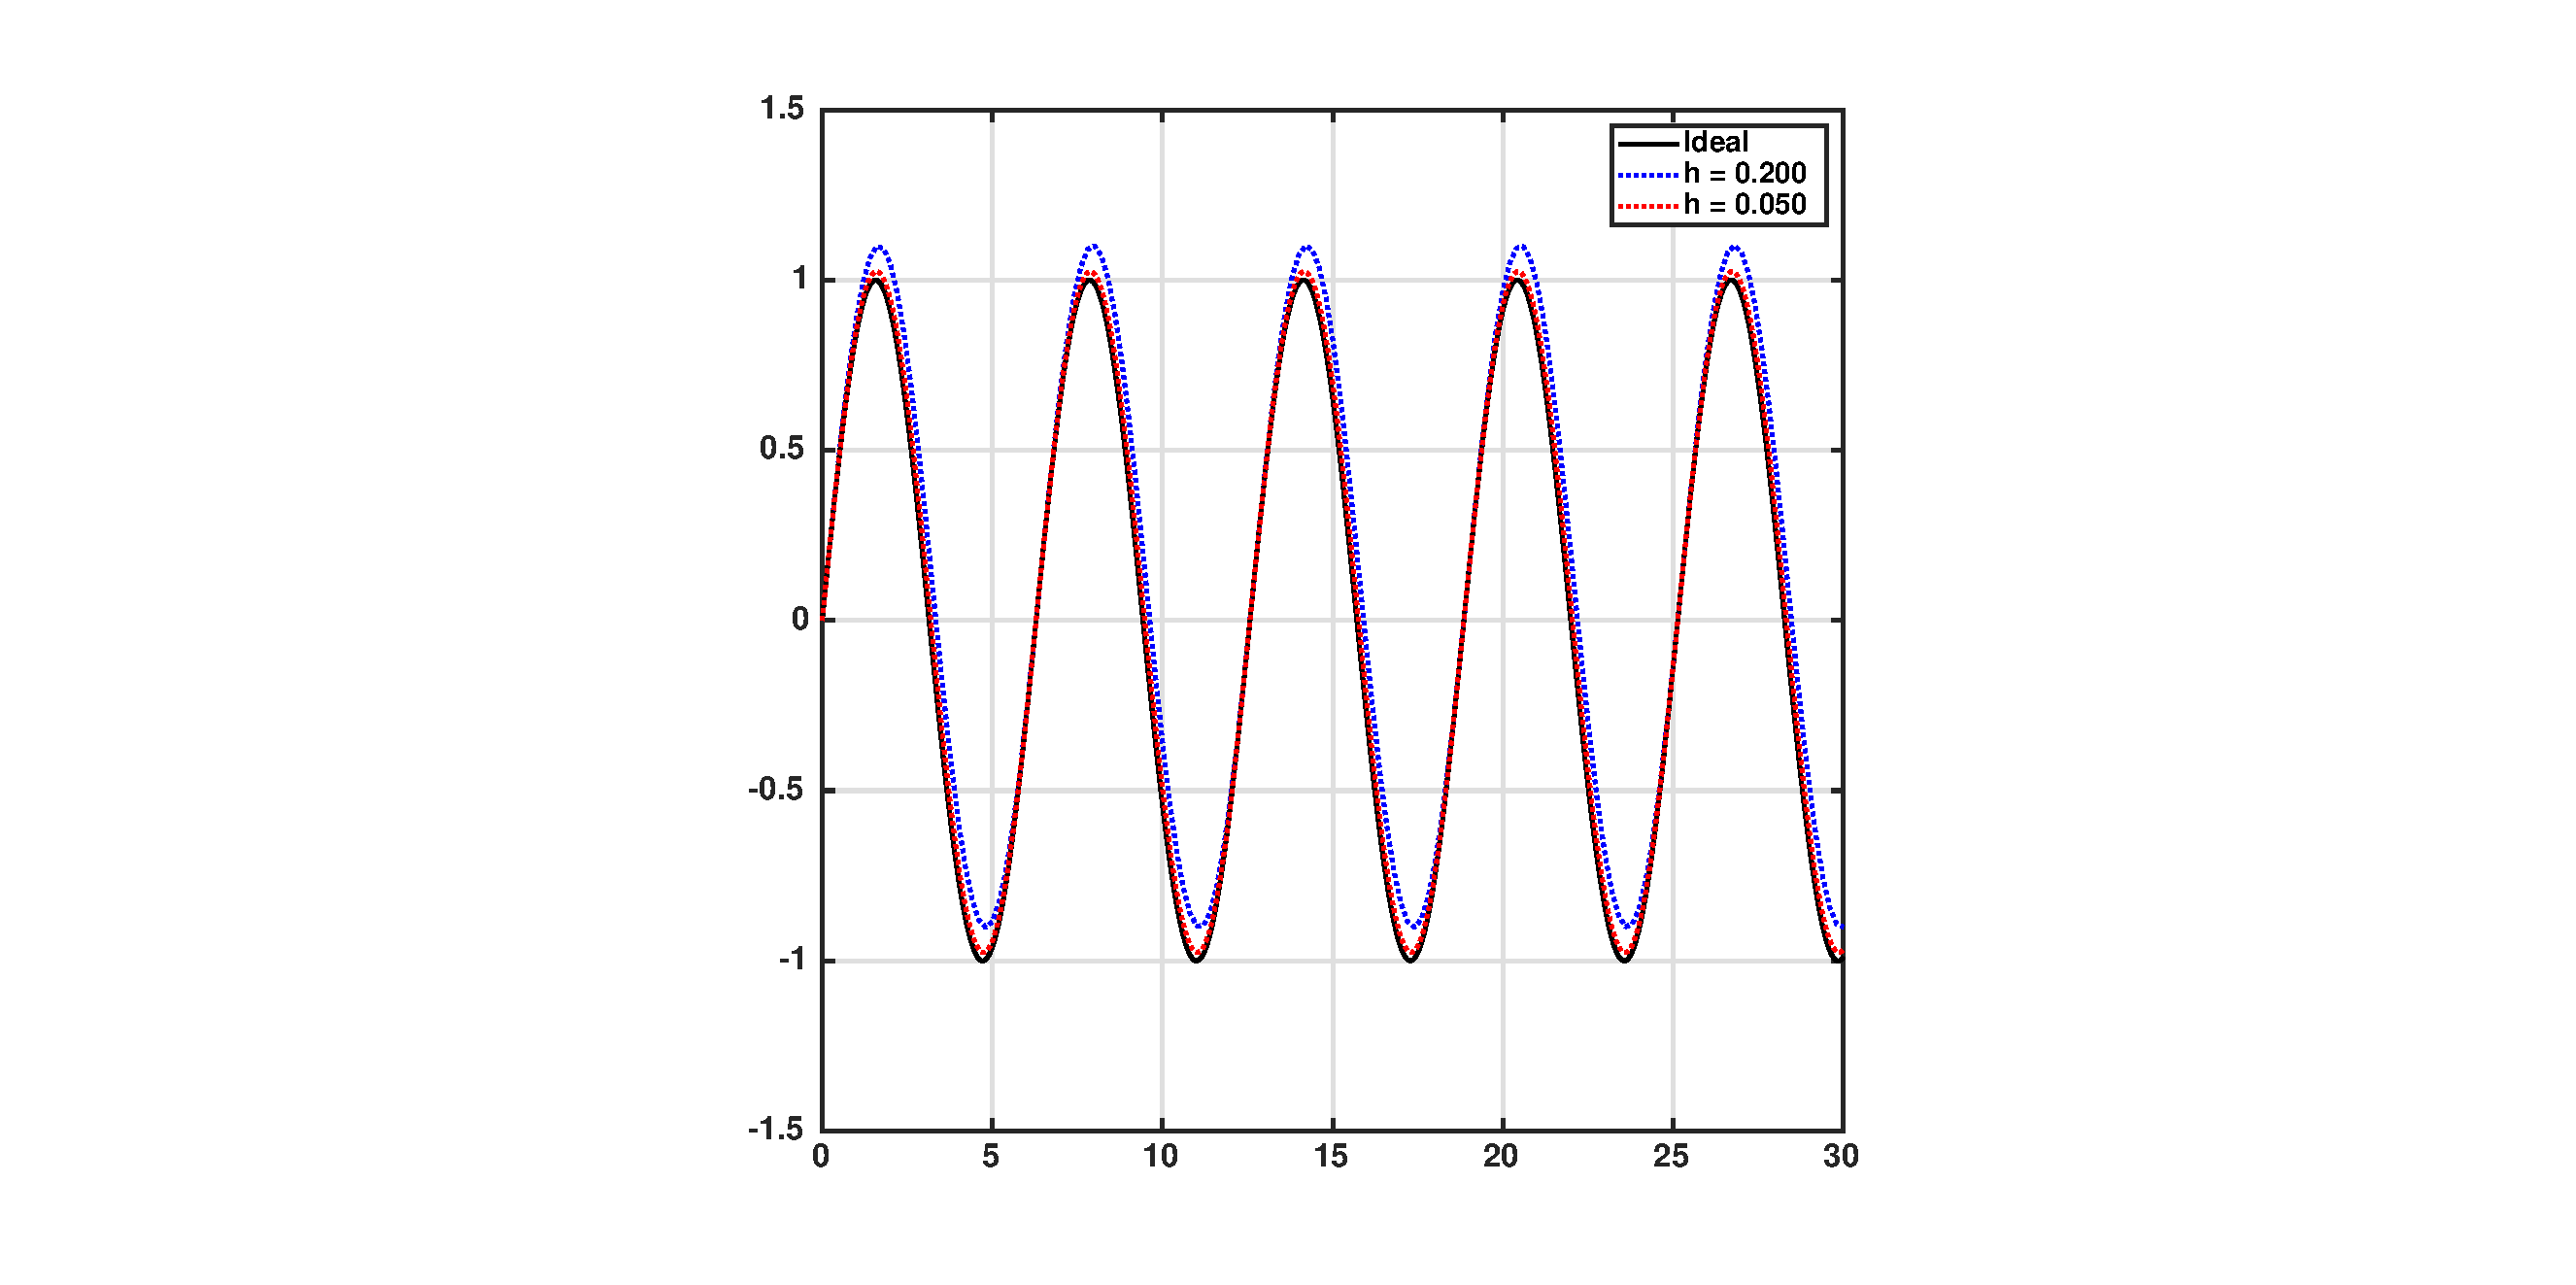
\includegraphics[trim=3in 0.3in 3in 0.3in, clip,scale=0.4]{ResearchNotes_TimePDE/figs/eulerTest.eps}
\caption{Numerical solution for the IVP with $\dot{y}(t)=\cos(t)$ and $y_{0}=0$ for different step sizes as compared to the ideal solution $y(t)=\sin(t)$.}
\label{fig:IVP1}
\end{figure}\begin{figure}[!t]
\centering
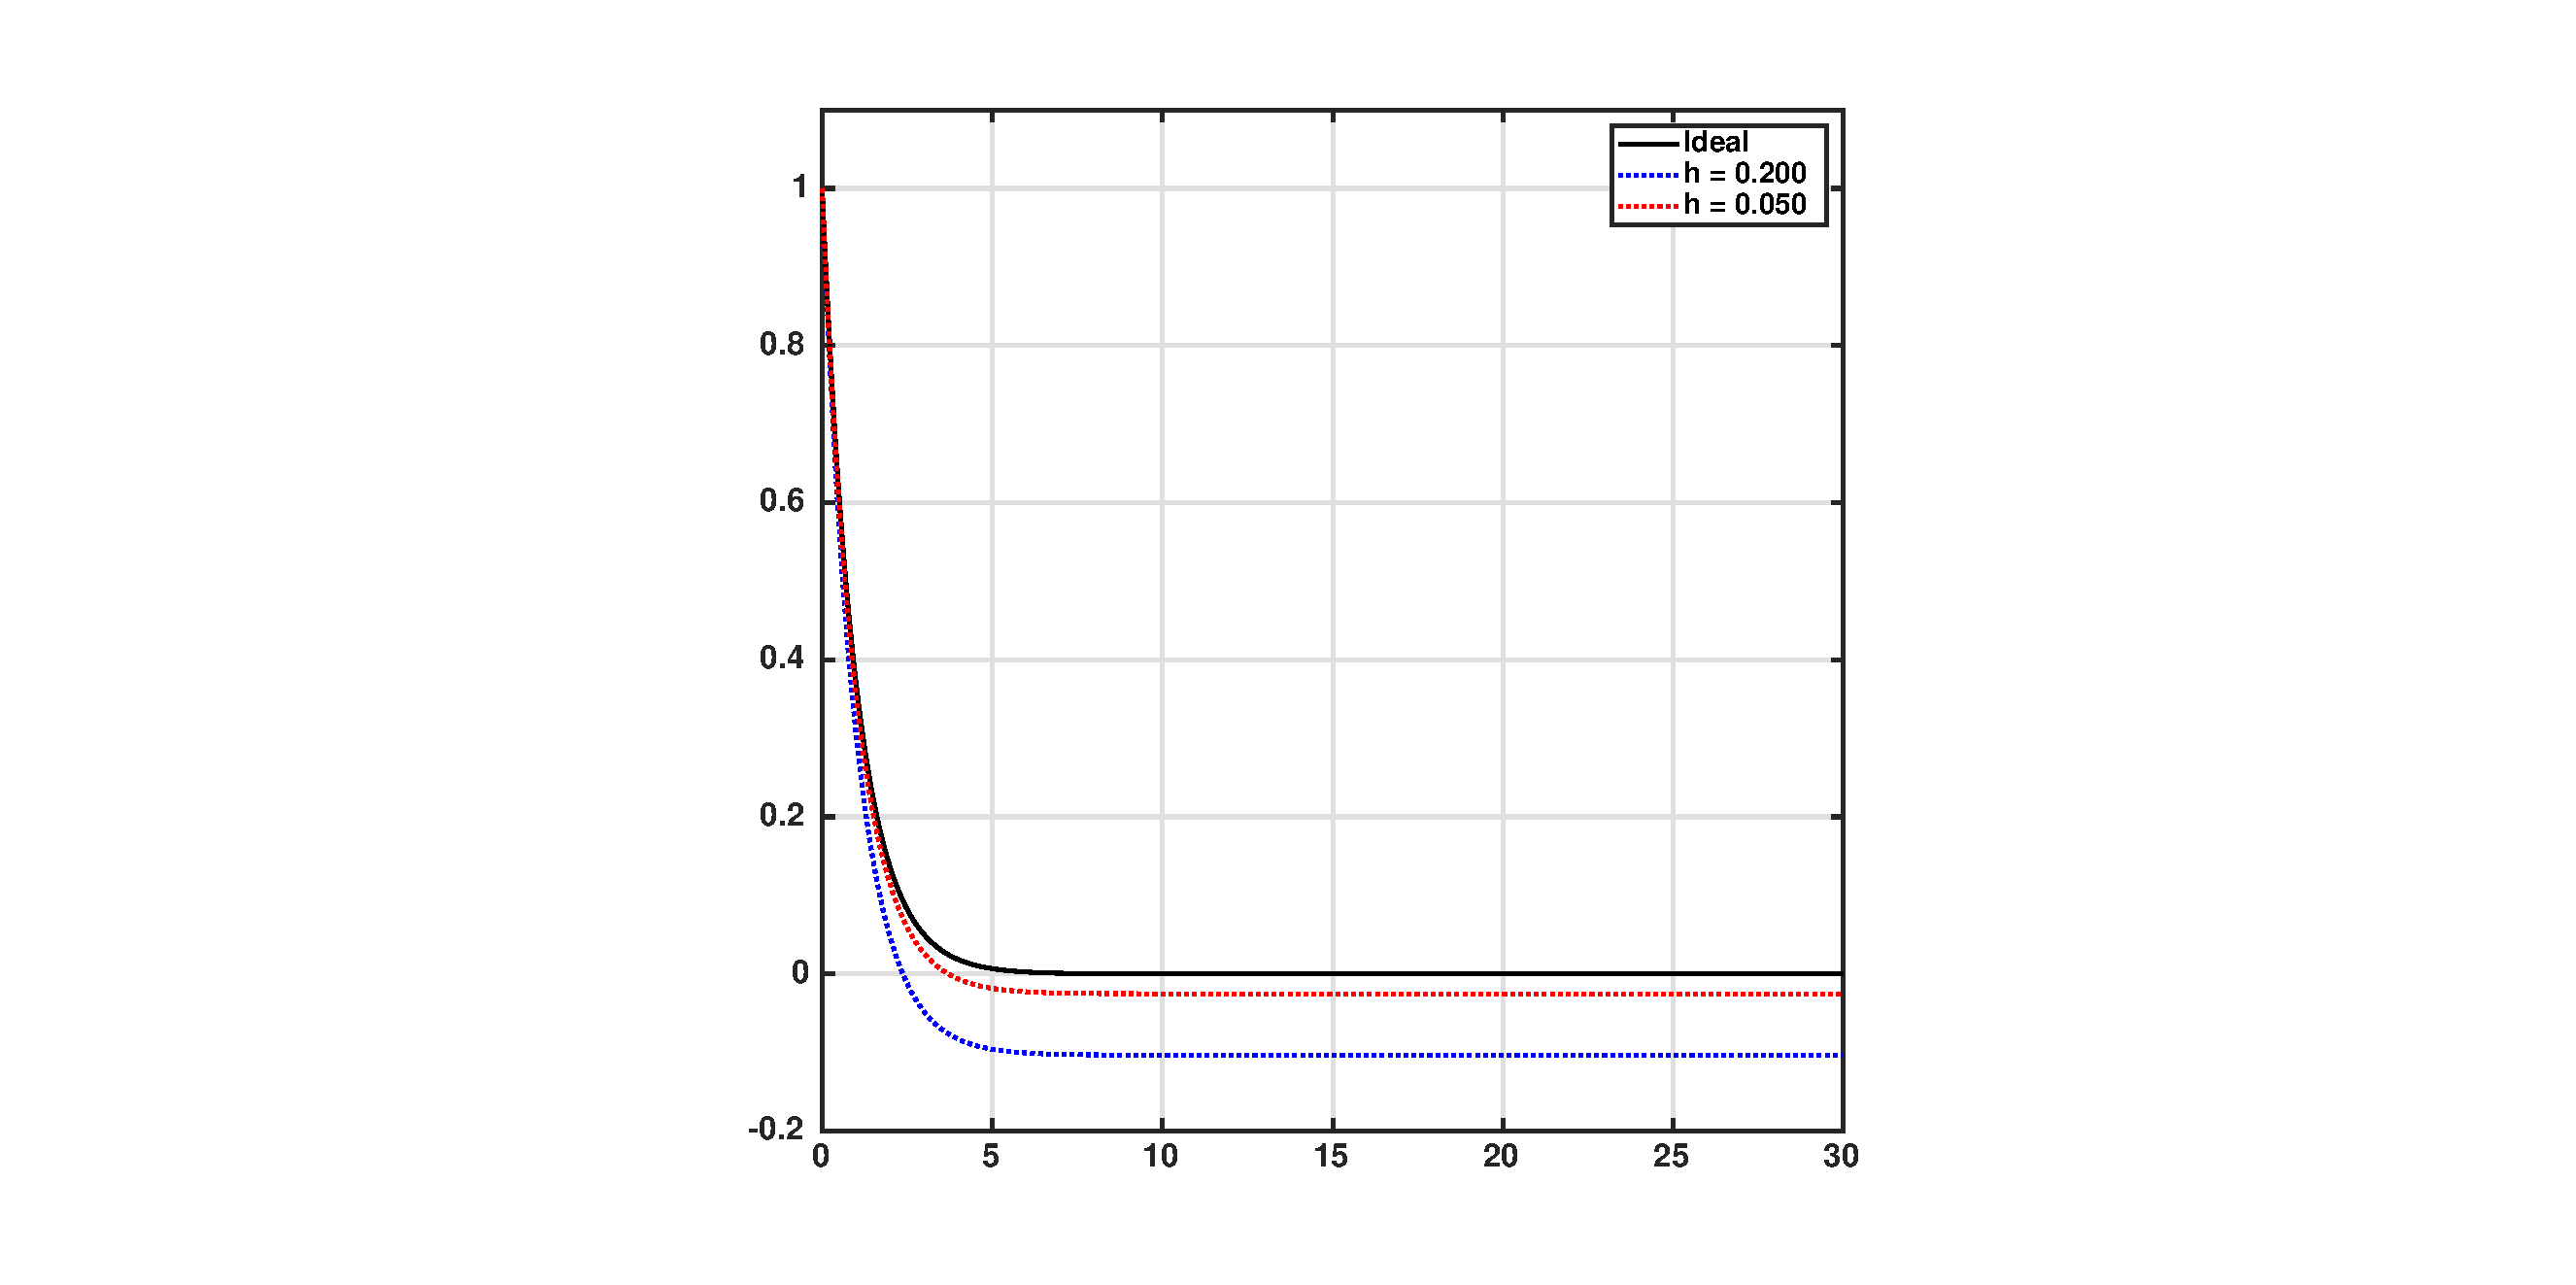
\includegraphics[trim=3in 0.3in 3in 0.3in, clip,scale=0.4]{ResearchNotes_TimePDE/figs/eulerTest2.eps}
\caption{Numerical solution for the IVP with $\dot{y}(t)=-\exp(-t)$ and $y_{0}=1.0$ for different step sizes as compared to the ideal solution $y(t)=\exp(-t)$.}
\label{fig:IVP2}
\end{figure}\clearpage
}

\section{Higher Order Explicit Methods}

Equation~(\ref{eq:simpExEuler}) has a similar form as the power series expansion, which is written as\begin{IEEEeqnarray}{rCl}
y(t) & = & \sum^{+\infty}_{n=0}a_{n}y^{(n)}(t)
\end{IEEEeqnarray}where the superscript $(n)$ denotes the $n$-th derivative of $y$. Thus, the forward Euler method may be thought of as a first order estimation for $y(t)$ and the full expression is\begin{IEEEeqnarray}{rCl}
y_{n+1} & = & y_{n} + hf(t,y_{n}) + \mathcal{O}(h^{2})
\end{IEEEeqnarray}and the error in using Equation~(\ref{eq:simpExEuler}) to approximate $y(t)$ is $\mathcal{O}(h^{2})$. By expanding the power series further, we can derive higher order explicit methods for $y_{n+1}$ and reduce the error.

\subsection{The Heun Method}

The Heun method is a second order method to approximate $y_{n+1}$ and is given by the expression\begin{IEEEeqnarray}{rCl}
y_{n+1} & = & y_{n} + h\frac{k_{1}+k_{2}}{2},~\text{where} \label{eq:heun} \\
k_{1} & = & f(t,y_{n}) \nonumber \\
k_{2} & = & f(t+h,y_{n}+hk_{1}) \nonumber
\end{IEEEeqnarray}It can be seen that $y_{n+1}$ is determined using two evaluations of $f()$ ($k_{1}$ and $k_{2}$). The evaluation of $k_{1}$ is akin to the explicit Euler method. The evaluation of $k_{2}$ occurs at the point predicted using the Euler method. The average of $k_{1}$ and $k_{2}$ is then used to estimate $y_{n+1}$.

\subsection{The 4-th Order Runge-Kutta (RK) Method}

German mathematicians Carl Runge and Wilhelm Kutta derived methods (also called Runge-Kutta methods or RK methods) to approximate $y_{n+1}$. The 4-th order RK method (RK4) is given by the expression\begin{IEEEeqnarray}{rCl}
y_{n+1} & = & y_{n} + \frac{h}{6}\left(k_{1}+2k_{2}+2k_{3}+k_{4}\right),~\text{where} \\
k_{1} & = & f(t,y_{n}) \nonumber \\
k_{2} & = & f\left(t+\frac{h}{2}, y_{n}+h\frac{k_{1}}{2}\right) \nonumber \\
k_{3} & = & f\left(t+\frac{h}{2}, y_{n}+h\frac{k_{2}}{2}\right) \nonumber \\
k_{4} & = & f(t+h,y_{n}+hk_{3}) \nonumber
\end{IEEEeqnarray}In this method $f()$ are evaluated at points within the time step to obtain a better approximation of $y_{n+1}$.

\subsection{The Butcher Tableau}

From the methods discussed so far, it can be seen that the general equation for determining $y_{n+1}$ is \begin{IEEEeqnarray}{rCl}
y_{n+1} & = & y_{n} + h\sum^{s}_{i=1}b_{i}k_{i},~\text{where} \\
k_{1} & = & f(t,y_{n}) \nonumber \\
k_{2} & = & f(t+c_{2}h,y_{n}+a_{21}k_{1}) \nonumber \\
k_{3} & = & f(t+c_{3}h,y_{n}+a_{31}k_{1}+a_{32}k_{2}) \nonumber \\
& \vdots & \\
k_{s} & = & f(t+c_{s}h, y_{n}+\sum^{s-1}_{j=1}a_{s,j}k_{j}) \nonumber
\end{IEEEeqnarray}The mathematician proposed a concise way of describing the numerical method for solving PDEs and ODEs using a tableau called the Butcher tableau.

From the earlier examples, we can see that:
\begin{figure}
\centering
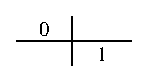
\includegraphics[scale=1.0]{ResearchNotes_TimePDE/figs/eulerButcher.eps}
\caption{Butcher Tableau for the Euler method.}
\end{figure}

\section{The Backward (Implicit) Euler Method}

\section{Adaptive time stepping}
